% lab_1.tex - Lab 1 for Cloud Computing class (Spring 2015)
% Chanmann Lim - November 2014

\documentclass[a4paper]{article}

\usepackage[margin=1 in]{geometry}
\usepackage{listings}
\usepackage{graphicx}

\begin{document}
\title{CS 7001-03: Report for Lab 1 - AWS Account Setup and Services Overview}
\author{Chanmann Lim\\ 
	\texttt{cl9p8@mail.mail.missouri.edu}}
\date{February 05, 2015}
\maketitle

\paragraph{1. } Screenshot of billing alarm setup: \\
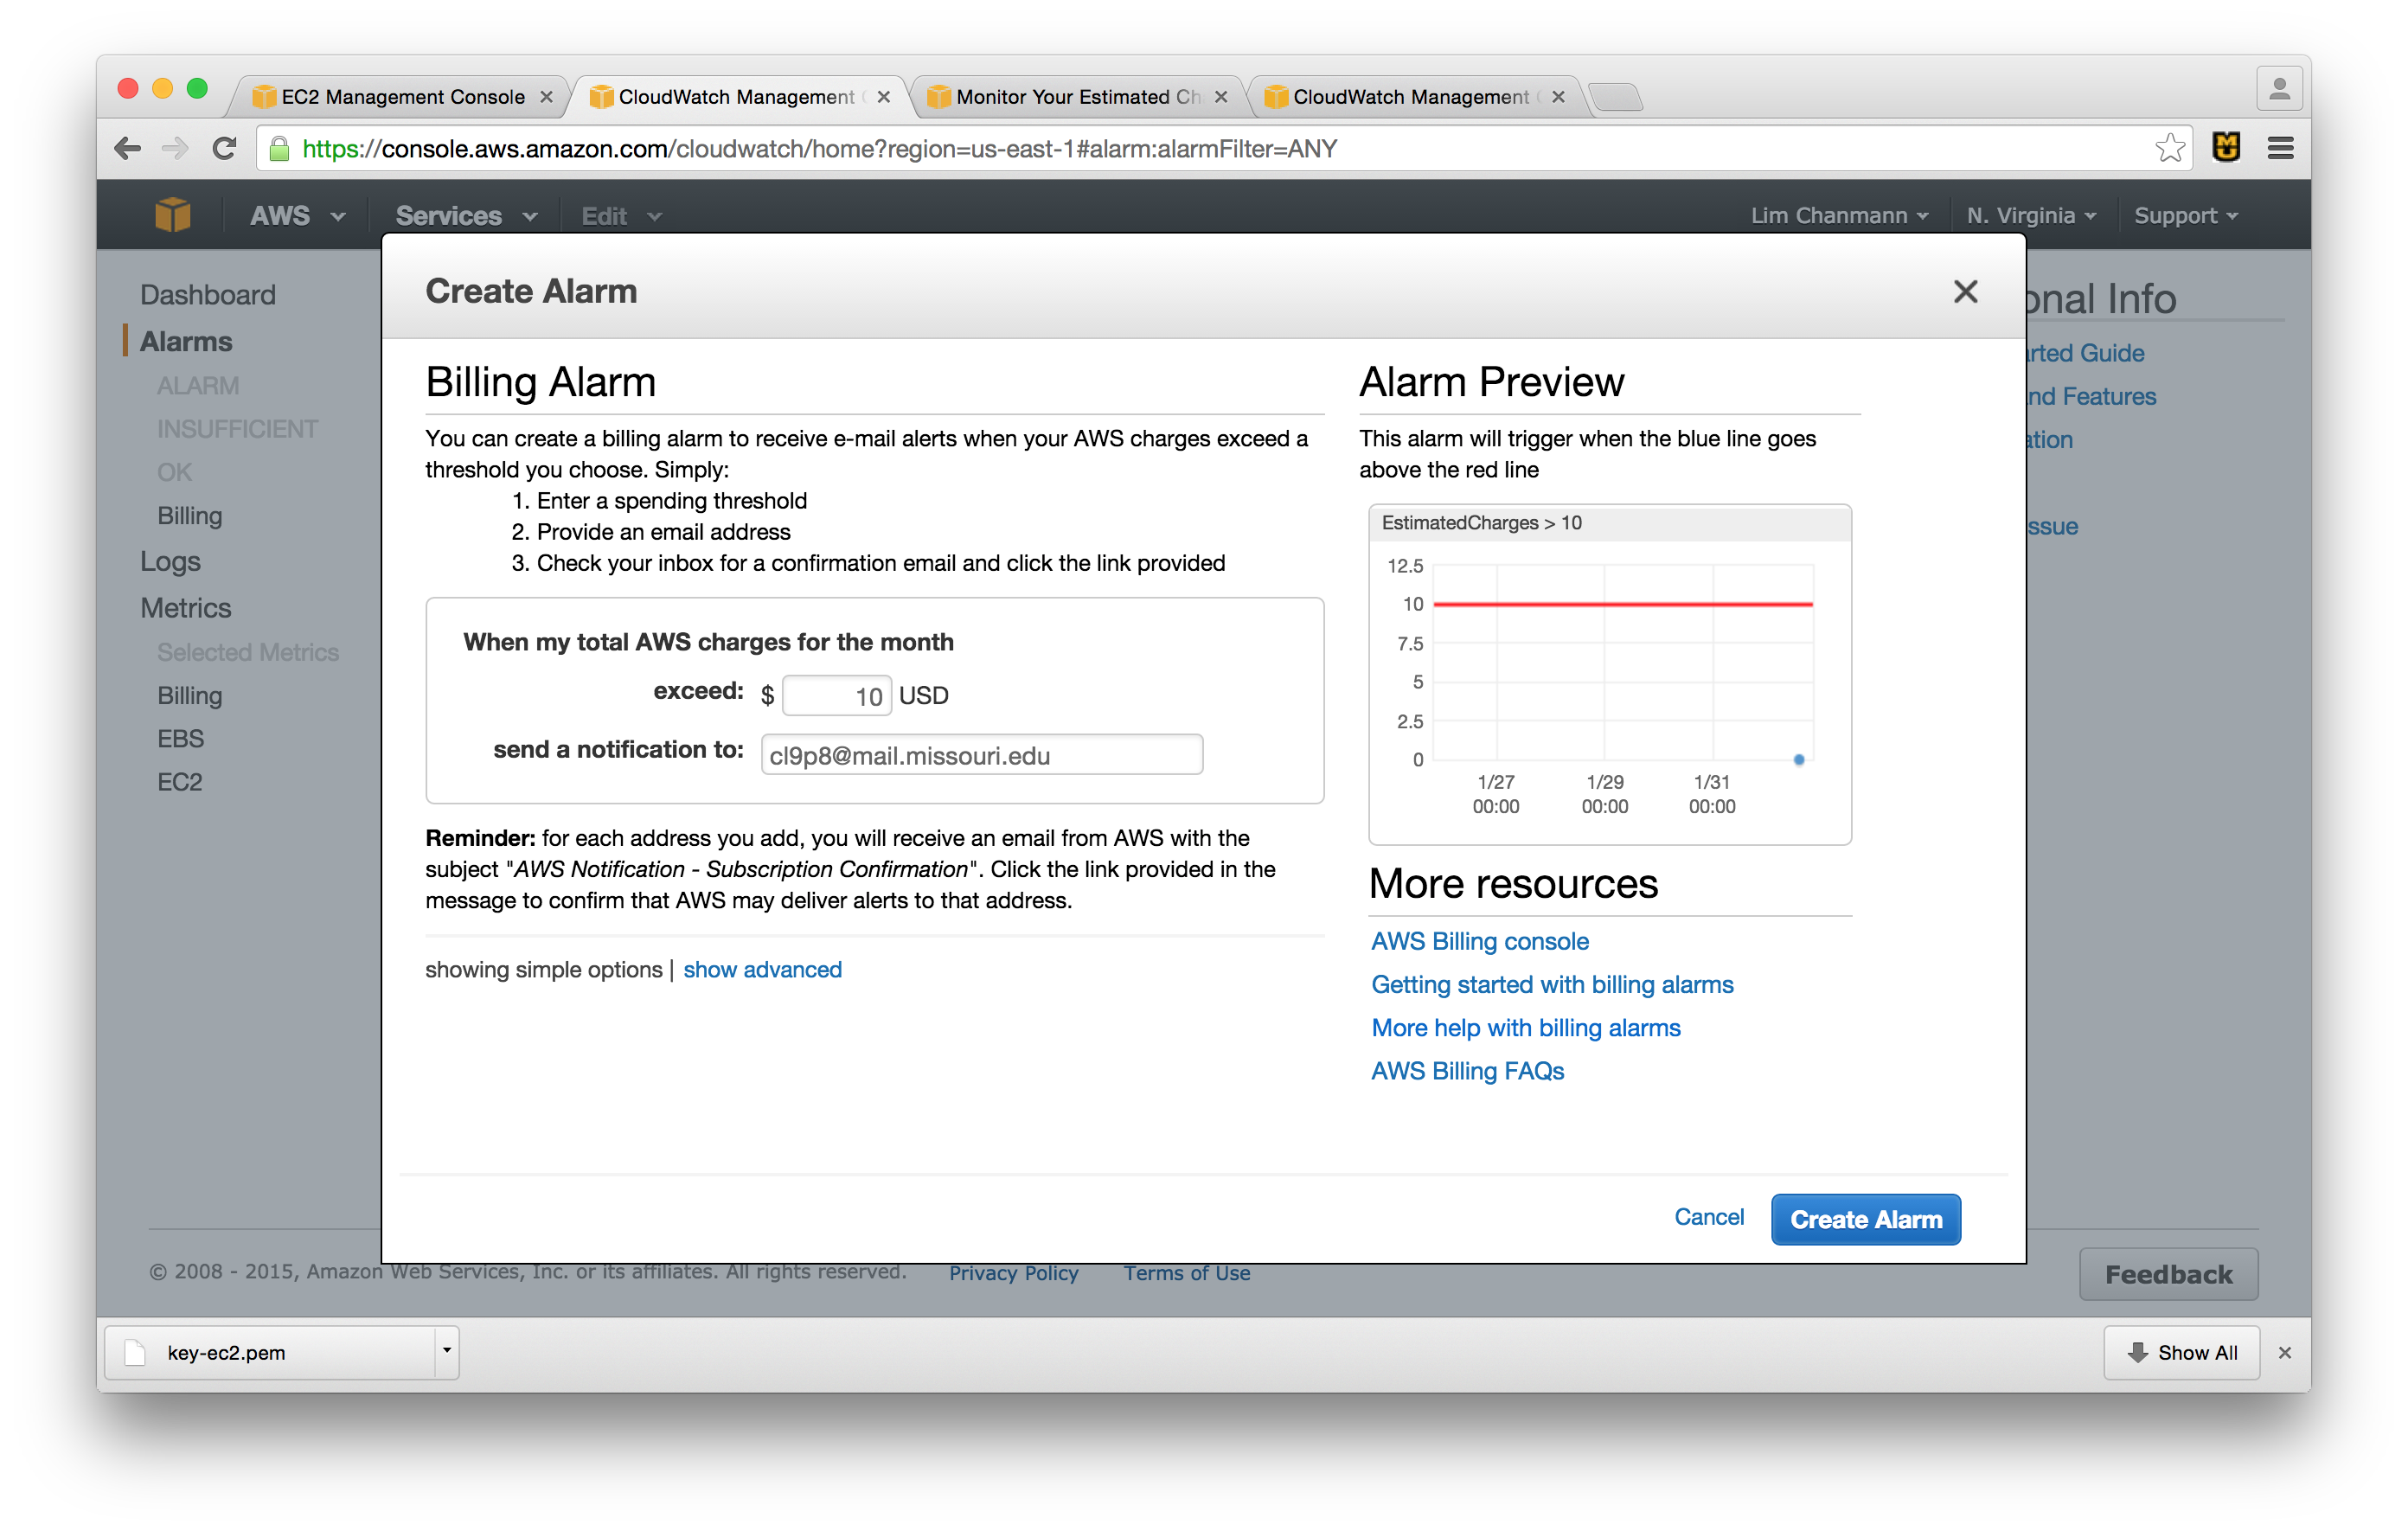
\includegraphics[scale=.32]{billing_alarm.png} \\

\paragraph{2. } List of AWS services by Categories:
\begin{description}
\leftskip 0.4in
\parindent -0.4in
	\item[Database: ] \hfill \\RDS \\DynamoDB \\ElastiCache \\RedShift
	\item[Storage \& CDN: ] \hfill \\S3 \\Storage Gateway \\Glacier \\CloudFront
	\item[Analytics: ] \hfill \\EMR \\Kinesis \\Data Pipeline
	\item[Compute \& Networking: ] \hfill \\EC2 \\VPC \\Direct Connect \\Route 53
	\item[Deployment \& Management: ] \hfill \\Elastic Beanstalk \\OpsWorks \\CloudFormation \\CodeDeploy
	\item[App Services: ] \hfill \\SQS \\AppStream \\SES \\CloudSearch
\end{description}

\paragraph{3. } Eight AWS services: \\




\end{document}